\section{Arquitetura Inicial}

De forma a perceber-se qual o comportamento do sistema como um todo, sem qualquer tipo de replicação ou otimização, decidiu-se fazer uma primeira instalação distribuída básica, utilizando \textit{Docker} e \textit{Docker Compose}, tendo por a configuração disponível na documentação do \textit{Wiki.js}, em \cite{wiki-docker}.

O objetivo desta instalação é conseguir avaliar o desempenho do sistema através da execução de um \textit{workload} com múltiplos testes de carga e, com base nos respetivos resultados, identificar e explorar os potenciais pontos críticos onde o sistema pode falhar ou perder desempenho.

Para tal, usou-se uma configuração de \textit{Docker Compose} com dois serviços (\textbf{\textit{db}} e \textbf{\textit{wiki}}), tal como se pode ver no anexo \ref{appendix:wiki-docker-compose}.

\subsection{Pontos Críticos do Sistema}

Para que seja possível garantir que um serviço possua uma elevada disponibilidade mantendo-se com um bom desempenho no atendimento de pedidos, torna-se necessário perceber quais são os \textbf{pontos críticos de falha e desempenho} do nosso sistema.

O principal cenário em que um sistema pode falhar é aquele em que um dos componentes que o constitui (ou mais) falhar, não existindo mais do que uma instância de cada um destes elementos. Isto pode acontecer quer por falhas de software/hardware, quer por falhas de energia. No nosso caso em concreto, com a nossa arquitetura inicial, possuímos 2 elementos: a \textbf{Base de Dados} e o servidor \textbf{Wiki.js}. Estes elementos não possuem qualquer réplica, o que significa que na eventualidade de um ou mais falhar, todo o sistema irá ficar inoperacional.

Outro dos principais pontos de falha e desempenho de uma aplicação são os \textbf{\textit{bottlenecks}}. Os \textit{bottlenecks} são situações em que um componente da aplicação limita todas as outras, diminuindo a performance do sistema. No nosso caso, o principal \textit{bottleneck} que identificámos é a \textbf{Base de Dados} visto que tanto serve pedidos do \textit{frontend} como do \textit{backend}. Dado que a nossa base de dados não está preparada com mecanismos de alta disponibilidade, prevemos que esta poderá a vir ser um ponto crítico do sistema.

Com estes pontos, ficámos com uma melhor noção do que poderá vir a ser um problema no nosso sistema, e quais serão algumas das soluções possíveis.

\subsection{Testes de Carga}

De modo a avaliar o desempenho da nossa instalação recorremos a \textbf{Testes de Carga} utilizando o \textbf{JMeter}. Utilizando GUI do \textit{JMeter} criámos 4 Testes que tentam simular um pouco do que será o funcionamento de uma \textit{Wiki} de um determinado produto ou serviço. Considerámos que no nosso cenário de teste utilizadores normais apenas consultam páginas enquanto que administradores têm a possibilidade de efetuar login e adicionar, editar ou remover páginas. Efetuámos essa segregação devido à diferença nos números de utilizadores e administradores, sendo os primeiros em número consideravelmente superior.

Os testes foram corridos no ambiente de linha de comandos de modo a poupar recursos das nossas máquinas, sendo que as limitações de hardware e as limitações relativas à \textbf{JVM} foram os principais obstáculos ao aumento da carga.

\subsubsection{Teste 1}

O Teste 1 visa representar o cenário mais básico: um utilizador aceder à página inicial da wiki. Para este teste irão ser utilizadas mais \textit{threads} do que nos restantes dado que num cenário real, o acesso à página inicial da wiki é o mais comum. Ao correr este teste é testado o seguinte método:

\begin{enumerate}
  \item GET /
\end{enumerate}

O teste foi corrido com 100, 1000, 5000 e 10000 \textit{threads} (utilizadores), sendo que recorremos aos relatórios gerados pelo \textit{JMeter} para apresentar os seguintes resultados. 

\begin{table}[h!]
\centering
    \begin{tabular}{ |c|c|c|c|  }
        \hline
        \multicolumn{4}{|c|}{Página Inicial} \\
        \hline
         Threads & Erro & Tempo Resposta Médio (ms) & \textit{Throughput (Trans./s)}\\
        \hline
        100   & 0.00\%   & 4129.90  & 17.51\\
        1000  & 0.00\%   & 11572.32 & 47.10\\
        5000  & 47.20\%  & 23539.35 & 98.41\\
        10000 & 67.87\%  & 24610.09 & 157.72\\
        \hline
    \end{tabular}
    \caption{Instalação Simples - Sumário do Teste 1}
    \label{table:1}
\end{table}

\vspace{2cm}

Analisando os dados da tabela, podemos verificar que com 100 e com 1000 utilizadores não obtemos nenhuma percentagem de erro. Ao subir para um valor na casa dos 5000 já começámos a obter uma percentagem significativa de erros, sendo que com 10000 essa percentagem é ainda superior. Esta percentagem de erros permite-nos ter uma perceção do limite da disponibilidade da instalação atual da aplicação. 

Ao aumentar o número de threads, verificámos também o aumento do \textit{Throughput} da aplicação, bem como do tempo de resposta médio aos pedidos. Este último valor é aquele que nos preocupa mais acerca do teste dado que também pode ser encarado como um indicador de performance do sistema. Mesmo em casos em que todos os pedidos são atendidos, o tempo de resposta é bastante elevado, como por exemplo, no caso de 1000 \textit{threads}, em que precisámos em média de 11.6 segundos para abrir a página inicial, algo que é inaceitável nos padrões atuais. Os tempos de resposta elevados em conjunto com a elevada taxa de erro significam que o nosso sistema não está a responder corretamente aos pedidos efetuados. 

\begin{figure}[ht!]
    \centering
    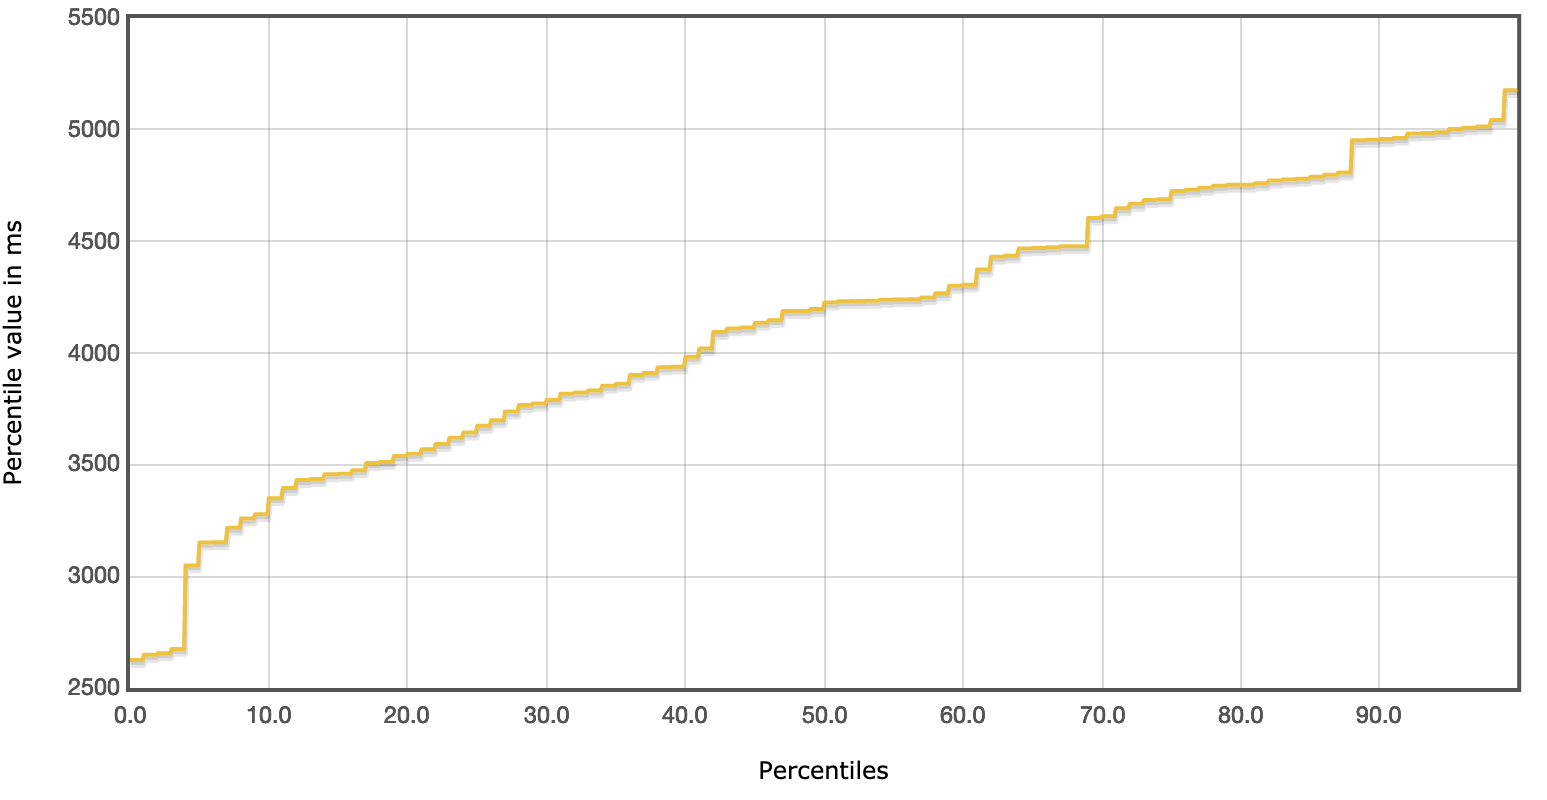
\includegraphics[width=.45\linewidth]{img/testes/i-t1-100.png}
    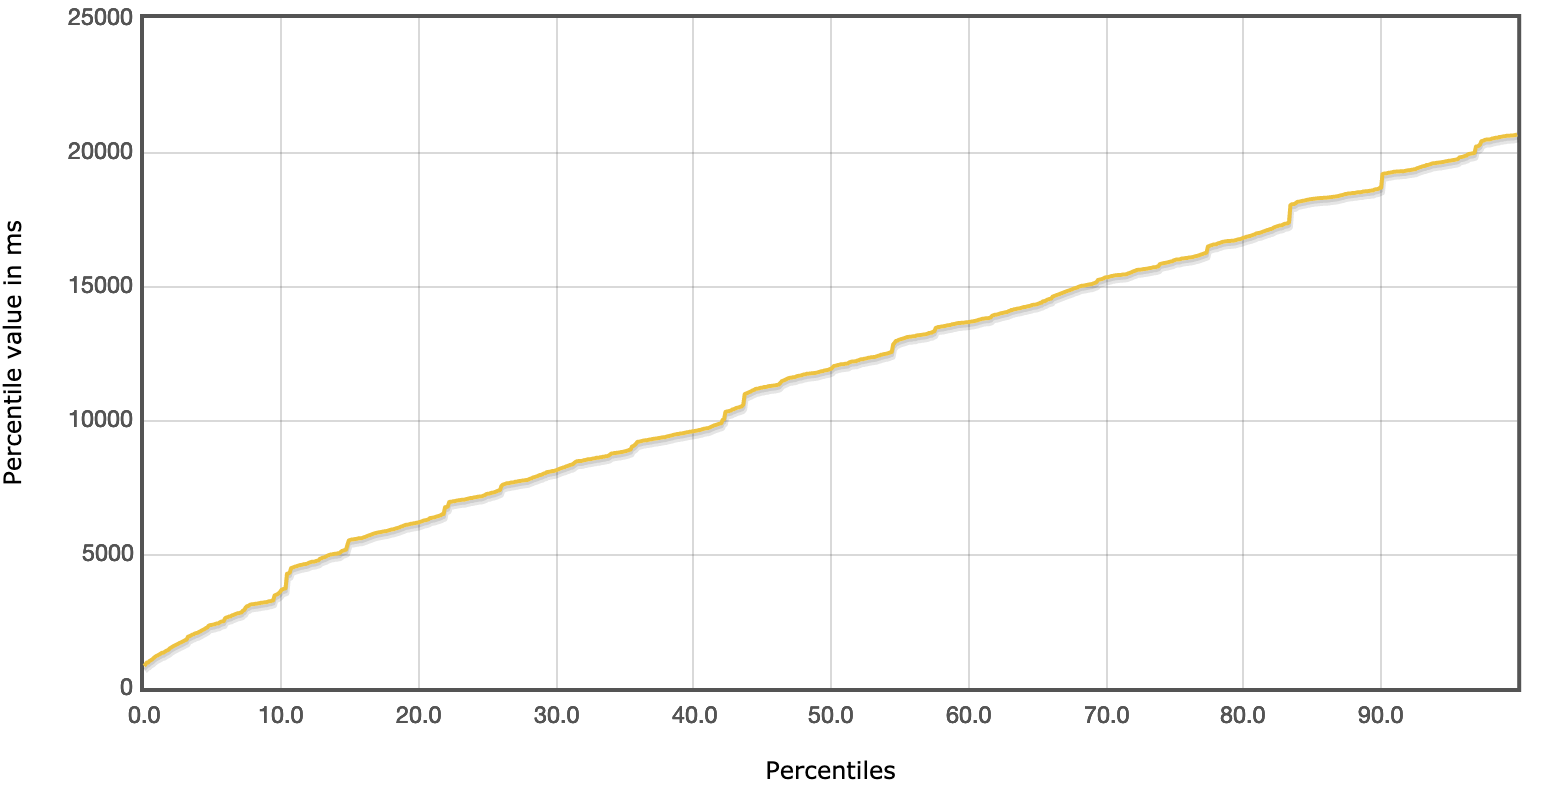
\includegraphics[width=.45\linewidth]{img/testes/i-t1-1000.png}
    \caption{Percentil Tempo de Resposta para 100 e 1000 Threads}
\end{figure}

\begin{figure}[ht!]
    \centering
    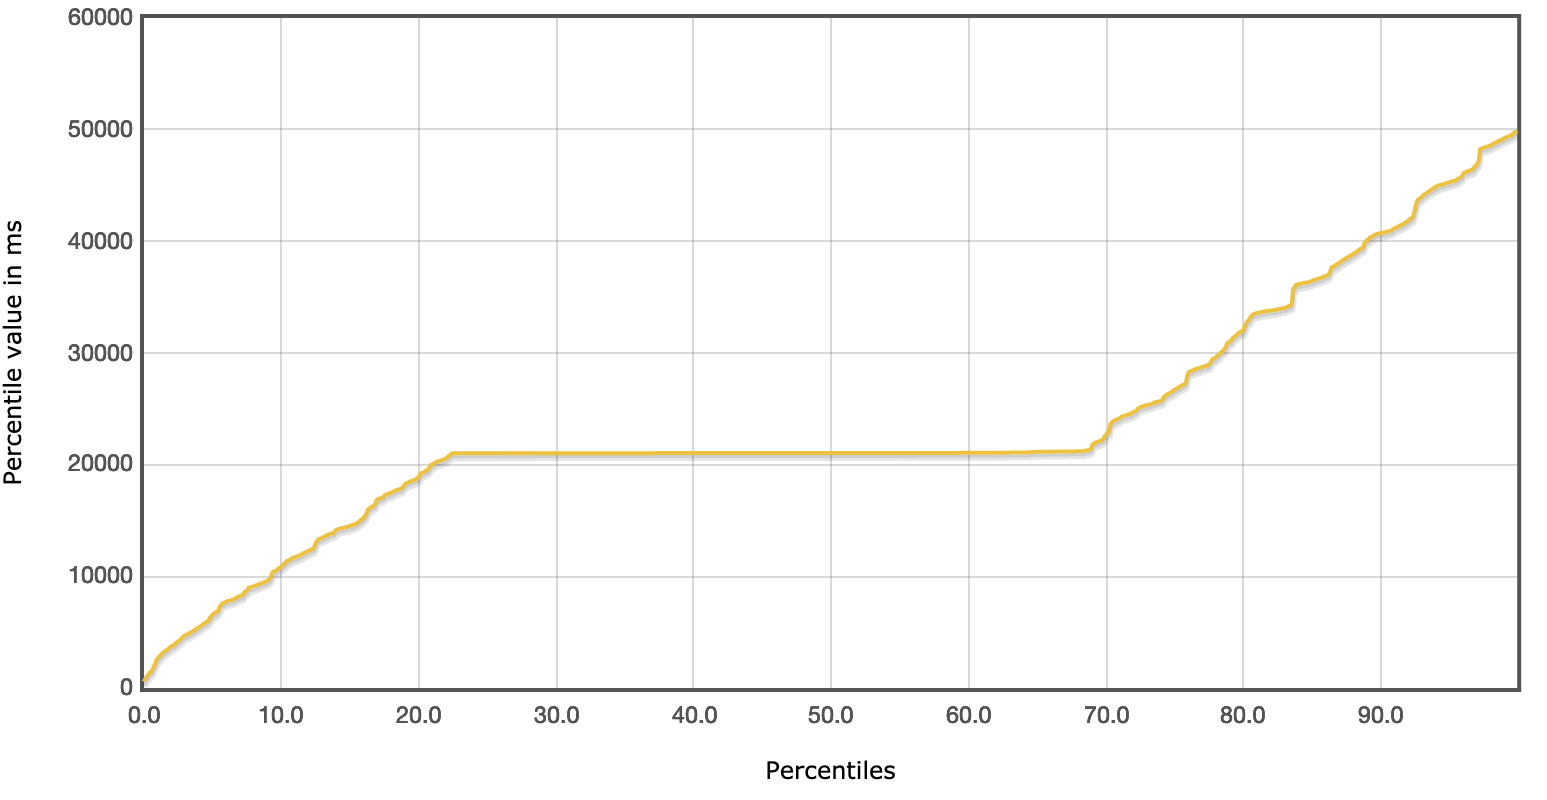
\includegraphics[width=.45\linewidth]{img/testes/i-t1-5000.png}
    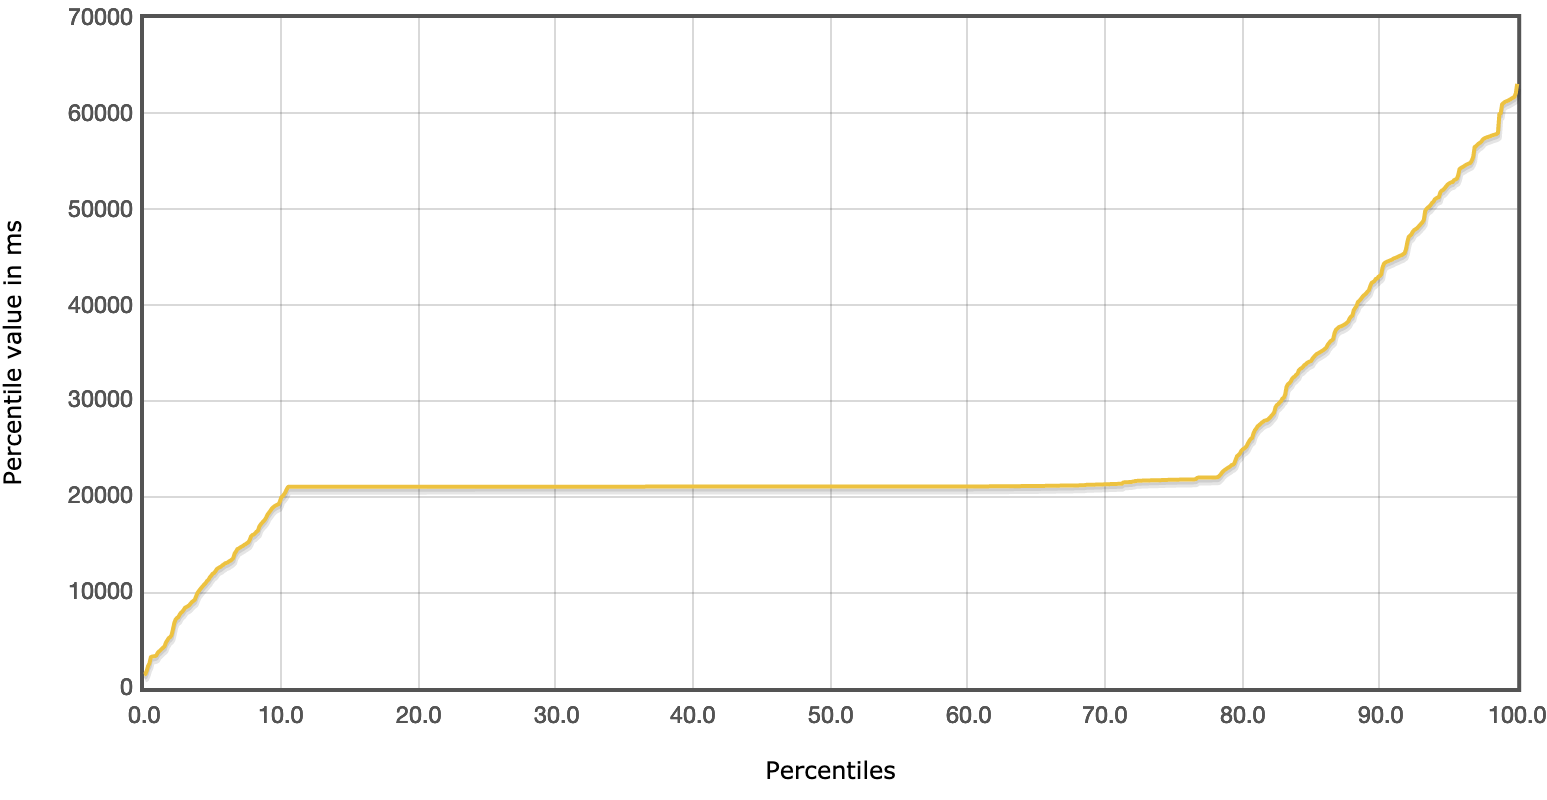
\includegraphics[width=.45\linewidth]{img/testes/i-t1-10000.png}
    \caption{Percentil Tempo de Resposta para 5000 e 10000 Threads}
\end{figure}

\vspace{2cm}
Verificando os gráficos apresentados, fica ainda mais evidente que os tempos de resposta da aplicação são bastante elevados.

\subsubsection{Teste 2}

O Teste 2 visa representar o cenário em que um utilizador entra na página inicial, navegando de seguida para uma outra página da wiki. Neste caso em específico, todas as \textit{threads} abrem a mesma página após pedirem a página inicial e esperarem 1000 milissegundos. Ao correr este teste são testados os seguintes métodos:

\begin{enumerate}
  \item GET /
  \item GET /en/ICD
\end{enumerate}

O teste foi corrido com 1000 e 5000 \textit{threads}, sendo que recorremos aos relatórios gerados pelo \textit{JMeter} para apresentar os seguintes resultados. Estes valores foram escolhidos pela sua relevância tendo em conta o teste anterior.

\begin{table}[h!]
\centering
    \begin{tabular}{ |c|c|c|c|c|  }
        \hline
        \multicolumn{4}{|c|}{Página Inicial} \\
        \hline
         Threads & Erro & Tempo Resposta Médio (ms) & \textit{Throughput (Trans./s)}\\
        \hline
        1000  & 0.00\%   & 9328.98  & 52.63\\
        5000  & 49.56\%  & 25202.86 & 109.55\\
        \hline
    \end{tabular}
    \caption{Instalação Simples - Sumário do Teste 2}
    \label{table:1}
\end{table}

Analisando os dados da tabela, podemos verificar que com 1000 utilizadores não obtemos nenhuma percentagem de erro. Quando aumentamos para valores na casa dos 5000 começámos a obter uma percentagem significativa de erros, que neste caso já se demonstra inaceitável para uma plataforma funcional. Esta percentagem de erros mostra-nos um pouco qual o limite da disponibilidade da aplicação de momento. 

Ao aumentar o número de threads, verificámos também o aumento do \textit{Throughput} da aplicação, bem como do tempo de resposta médio aos pedidos. Este último valor, dado que também serve de medida de performance do sistema, mostra-nos que nos casos em que assegurámos que todos os pedidos são atendidos, estes esperam uma quantidade de tempo considerável. 

\begin{figure}[ht!]
    \centering
    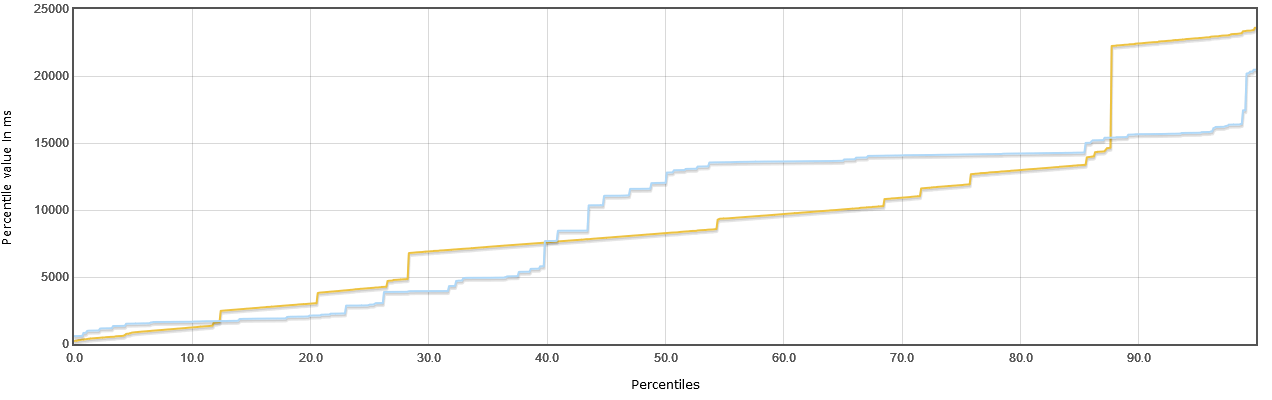
\includegraphics[width=.45\linewidth]{img/testes/i-t2-1000.png}
    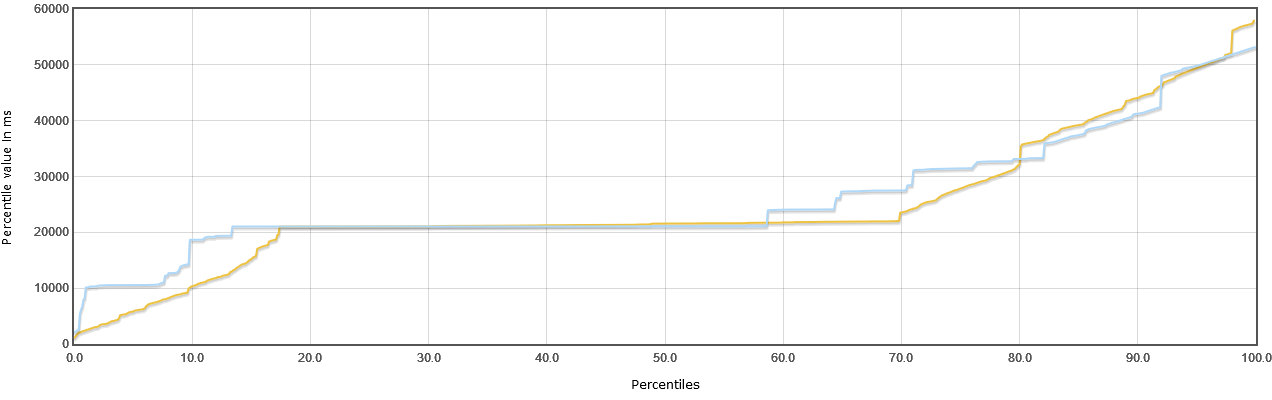
\includegraphics[width=.45\linewidth]{img/testes/i-t2-5000.png}
    \caption{Percentil Tempo de Resposta para 1000 e 5000 Threads}
\end{figure}

Verificando os gráficos apresentados, em que a linha azul representa os pedidos referentes à página de teste e a linha laranja os pedidos referentes à página inicial, fica ainda mais evidente que os tempos de resposta da aplicação são bastante elevados.

\subsubsection{Teste 3}

O Teste 3 visa representar o cenário em que um administrador efetua login no sistema, sendo redirecionado para a página principal. Ao correr este teste são testados os seguintes métodos:

\begin{enumerate}
  \item GET  /login
  \item POST /graphql
  \item GET  /
\end{enumerate}

O teste foi corrido com 100, 250, 500, 1000 e 5000 \textit{threads}, sendo que recorremos aos relatórios gerados pelo JMeter para apresentar os seguintes resultados.
O processo de login é constituido pelos 3 pedidos apresentados, sendo que o conteúdo do POST que é feito possui o endereço de email e a password da conta utilizada no teste. Estes 3 pedidos foram encapsulados num processo mais generalizado que representa o login como um todo. Optámos por esta visão de modo a representar de modo mais fidedigno o ato de efetuar login, dado que não é possível efetuar login se uma das operações falhar. Outra atenção que tivemos, foi o cancelamento de uma \textit{thread} no caso de um dos pedidos falhar.

\begin{table}[h!]
\centering
    \begin{tabular}{ |c|c|c|c|c|  }
        \hline
        \multicolumn{4}{|c|}{Página Inicial} \\
        \hline
         Threads & Erro & Tempo Resposta Médio (ms) & \textit{Throughput (Trans./s)}\\
        \hline
        100   & 0.00\%   & 6205.00  & 14.13\\
        250   & 0.00\%   & 7104.55  & 28.19\\
        500   & 0.00\%   & 16982.52 & 25.65\\
        1000  & 1.09\%   & 30312.79 & 22.80\\
        5000  & 64.74\%  & 90830.34 & 25.57\\
        \hline
    \end{tabular}
    \caption{Instalação Simples - Sumário do Teste 3}
    \label{table:1}
\end{table}

Analisando os dados da tabela, podemos verificar que com 100, 250 e 500 não obtemos nenhuma percentagem de erro. Ao subir para valor na casa dos 1000 já começámos a obter uma percentagem de erros, embora insignificativa. Nos 5000 utilizadores, a maioria deles já não consegue efetuar login. Esta percentagem de erros mostra-nos um pouco qual o limite da disponibilidade da aplicação de momento. 

Ao aumentar o número de threads, verificámos também o aumento do \textit{Throughput} da aplicação até um certo ponto, sendo que estagnou um pouco ao chegar às 500 threads. O tempo de resposta médio aos pedidos por sua vez não estagnou, subindo para valores elevados, mesmo sem a ocorrência de erros.

Nos gráficos apresentados, as \textbf{linhas vermelhas} representam o pedido \textbf{GET /login}, as \textbf{linhas azuis} representam o pedido \textbf{POST /graphql}, as \textbf{linhas amarelas} representam o pedido \textbf{GET /} e as \textbf{linhas verdes} representam o \textbf{Login} como um todo. Através destes gráficos, fica ainda mais evidente que os tempos de resposta da aplicação são bastante elevados.



\begin{figure}[ht!]
    \centering
    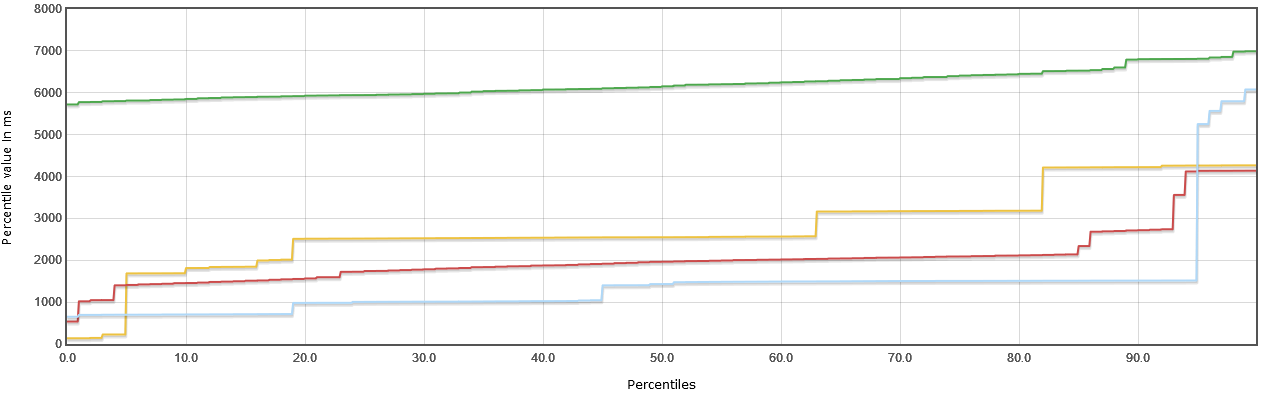
\includegraphics[width=.45\linewidth]{img/testes/i-t3-100.png}
    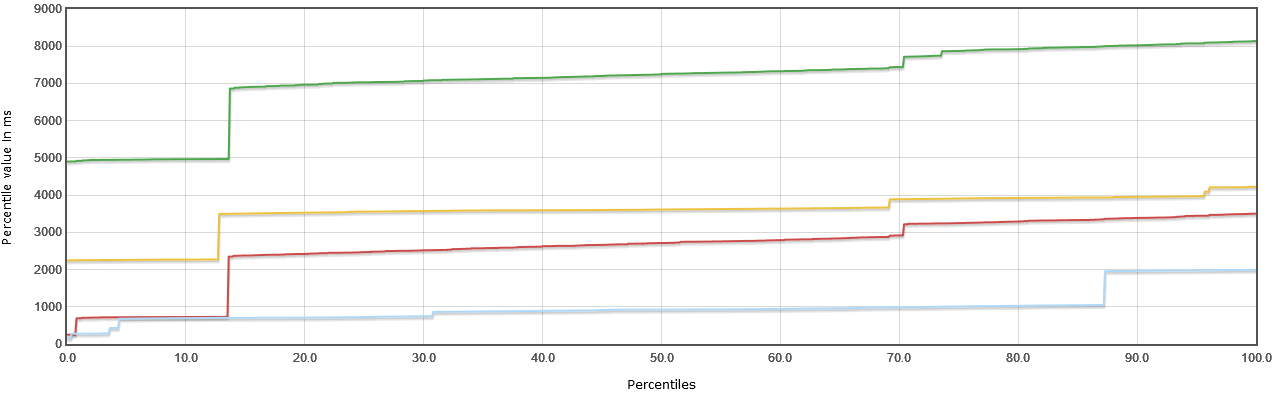
\includegraphics[width=.45\linewidth]{img/testes/i-t3-250.png}
    \caption{Percentil Tempo de Resposta para 100 e 250 Threads}
\end{figure}

\begin{figure}[ht!]
    \centering
    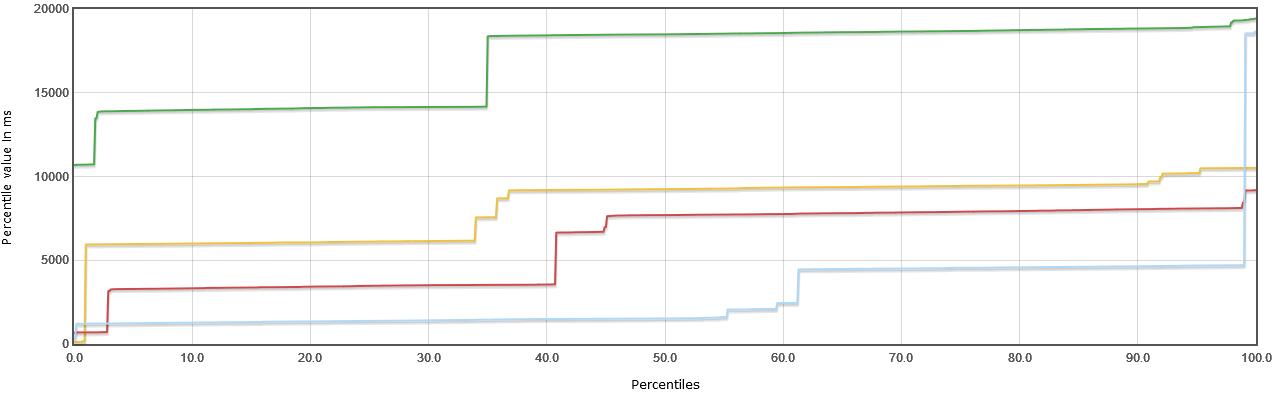
\includegraphics[width=.45\linewidth]{img/testes/i-t3-500.png}
    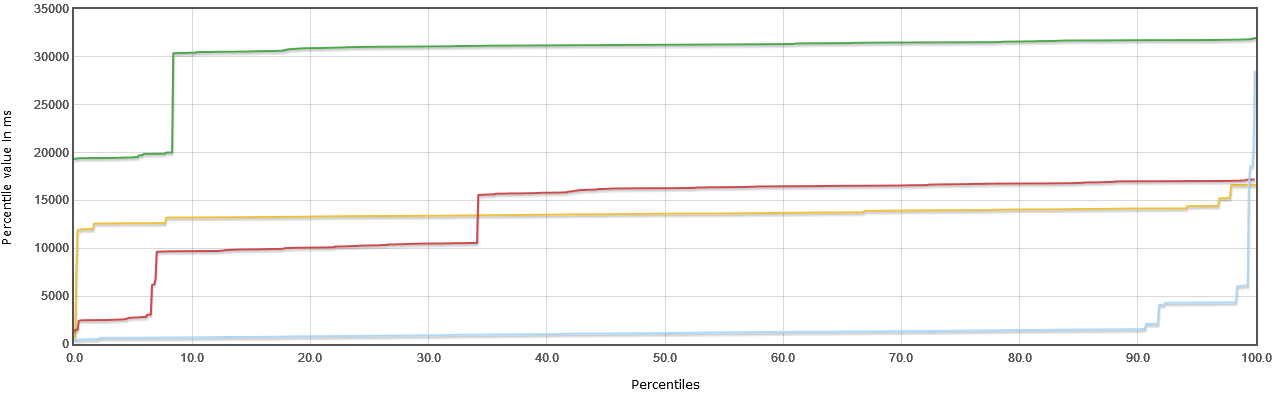
\includegraphics[width=.45\linewidth]{img/testes/i-t3-1000.png}
    \caption{Percentil Tempo de Resposta para 500 e 1000 Threads}
\end{figure}

\begin{figure}[ht!]
    \centering
    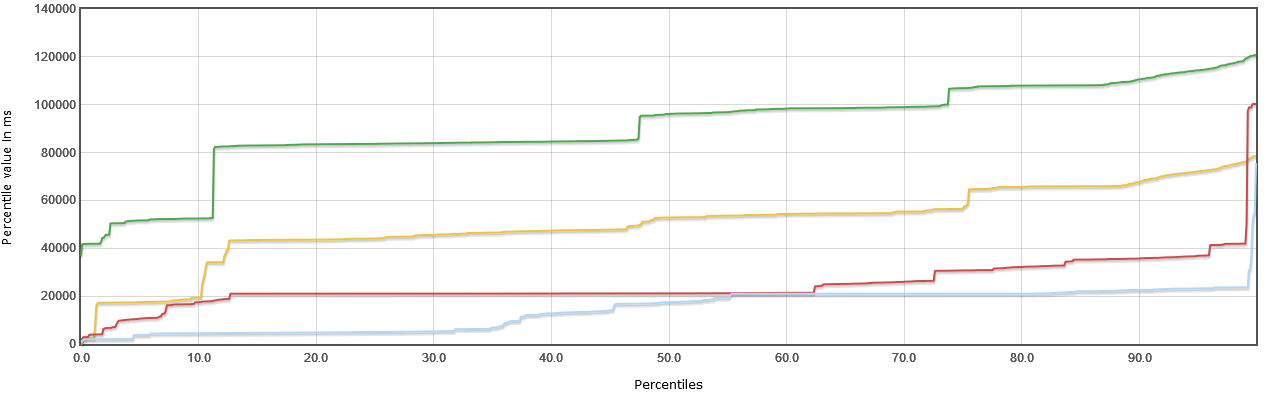
\includegraphics[width=.9\linewidth]{img/testes/i-t3-5000.png}
    \caption{Percentil Tempo de Resposta para 5000 Threads}
\end{figure}

% Para não haver texto a ir para espaços entre imagens
\pagebreak

\subsubsection{Teste 4}

O Teste 4 visa representar o cenário em que um administrador efetua login no sistema, sendo redireccionado para a página principal, seguido da criação de uma nova página wiki. Ao correr este teste são testados os seguintes métodos:

\begin{enumerate}
    \item GET /login
    \item POST /graphql
    \item GET /
    \item GET /e/en/ThreadNum-Pagename
    \item POST /graphql
    \item GET /e/en/ThreadNum-Pagename
\end{enumerate}

Nos métodos podemos encontrar as palavras \textit{ThreadNum} e \textit{Pagename}, que na verdade são variáveis. Cada \textit{thread} onde corremos os testes terá um \textit{ThreadNum} único, de maneira a conseguirmos saber que páginas cada \textit{thread} criou, e optamos por dar o nome à página a data do momento em que é criada em milissegundos para sabermos quando e por que ordem foram criadas as novas páginas. Isto é possível tomando partido das funções \texttt{\_\_time()} e \texttt{\_\_threadNum} do \textit{JMeter}.

O teste foi corrido com 100, 250 e 500 \textit{threads}, sendo que recorremos aos relatórios gerados pelo \textit{JMeter} para apresentar os seguintes resultados. A única diferença entre este teste e o anterior é que agora criamos uma página nova depois de fazermos o login, enquanto que no outro o teste acabaria precisamente depois de realizarmos o login. O processo de criação duma nova página é constituído pelos 3 últimos pedidos apresentados, sendo que o conteúdo do POST possui o conteúdo que a nova página irá apresentar. Estes 3 pedidos foram encapsulados num processo mais generalizado que representa a criação duma nova página como um todo. Optámos por esta visão de modo a representar de modo mais fidedigno o ato de criar uma nova página, dado que não é possível criá-la se uma das operações falhar. Sendo assim, preferimos separar a operação de efetuar login da criação da nova página para podermos avaliar individualmente cada um dos processos. 

\begin{table}[H]
\centering
\begin{tabular}{|c|c|c|p{3.5cm}|p{3cm}|}
\hline
Threads              & Operação & Erro    & Tempo Resposta Médio (ms) & \textit{Throughput (Trans./s)} \\ \hline
\multirow{2}{*}{100} & Login    & 0.00\%  & 4686.52                   & 17.05                          \\
                     & New Page & 18.00\% & 244610.95                 & 0.40                           \\ \hline
\multirow{2}{*}{250} & Login    & 0.00\%  & 12209.70                  & 18.49                          \\
                     & New Page & 37.14\% & 369123.91                 & 0.46                           \\ \hline
\multirow{2}{*}{500} & Login    & 0.00\%  & 23461.58                  & 19.98                          \\
                     & New Page & 84.25\% & 345850.68                 & 1.30                           \\ \hline
\end{tabular}
\caption{Instalação Simples - Sumário do Teste 4}
\end{table}

Analisando os dados da tabela, podemos verificar que as operações de login não possuem qualquer erro, enquanto que as da criação de páginas apresentam sempre erros, aumentando com o número de \textit{threads}. Podemos dizer que os tempos de resposta também aumentam proporcionalmente com o número de \textit{threads} mas o \textit{throughput} fica estagnado, seja qual for a operação e também o número de \textit{threads}!

Nos gráficos apresentados, as linhas \textbf{vermelho-escuro, roxo e amarelo-escuro} são as mais visíveis e ao mesmo tempo preocupantes, representando o \textbf{login, New Page e GET Page}, respetivamente. 

\begin{figure}[ht!]
    \centering
    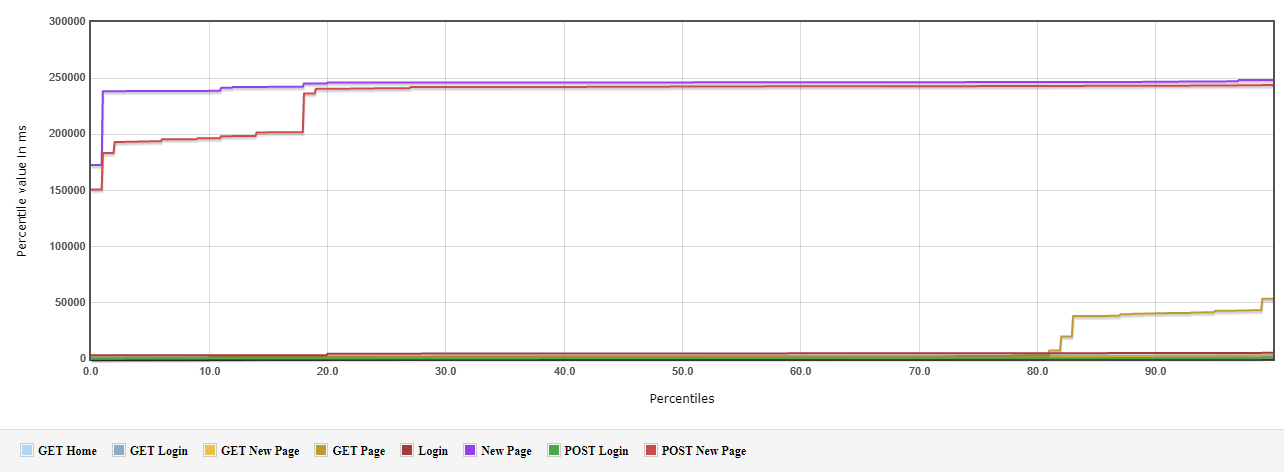
\includegraphics[width=.9\linewidth]{img/testes/i-t4-100.png}
    \caption{Percentil Tempo de Resposta para 100 Threads}
\end{figure}

\begin{figure}[ht!]
    \centering
    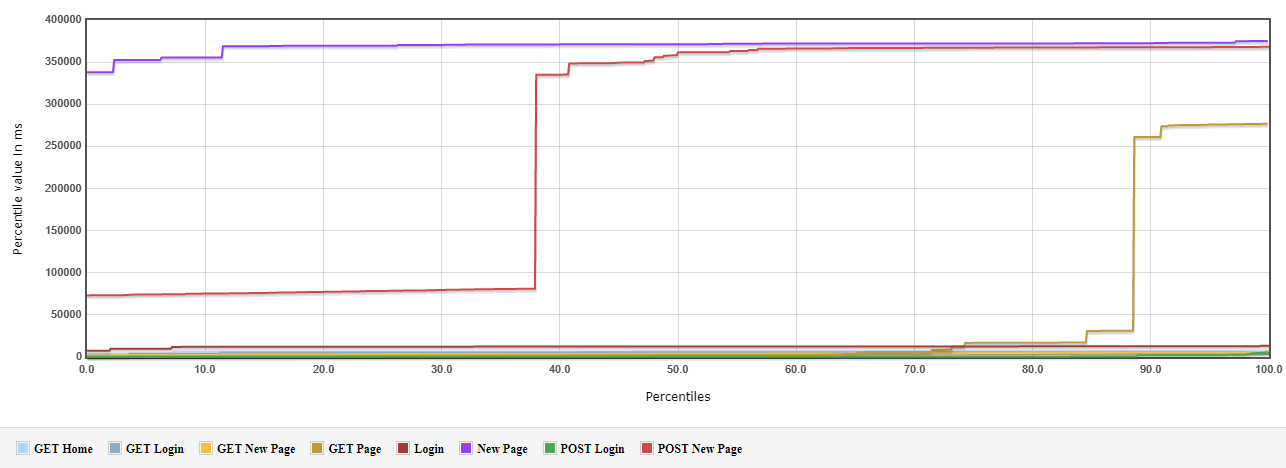
\includegraphics[width=.9\linewidth]{img/testes/i-t4-250.png}
    \caption{Percentil Tempo de Resposta para 250 Threads}
\end{figure}

\begin{figure}[ht!]
    \centering
    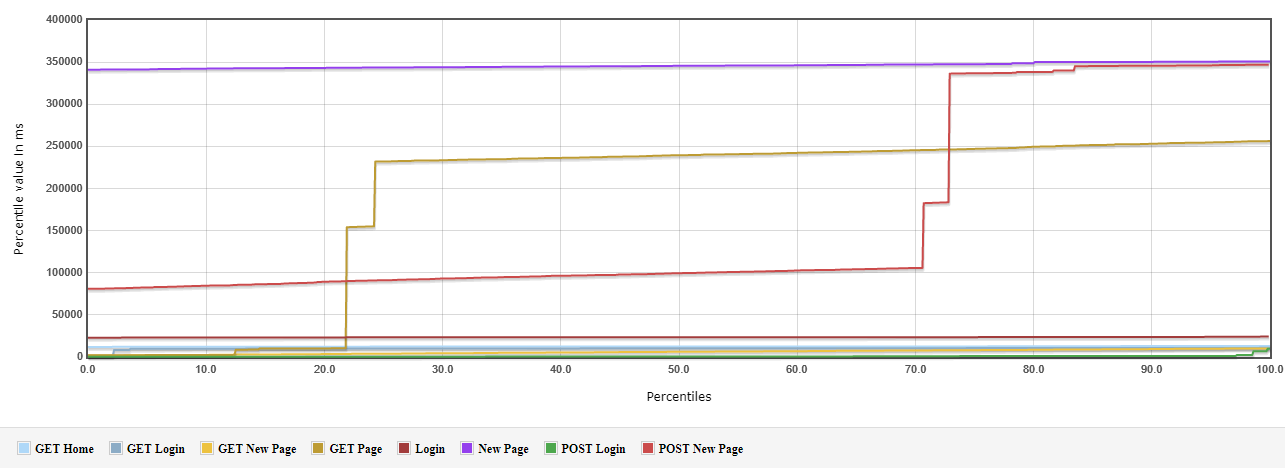
\includegraphics[width=.9\linewidth]{img/testes/i-t4-500.png}
    \caption{Percentil Tempo de Resposta para 500 Threads}
\end{figure}

\subsection{Análise de Desempenho}

Após analisarmos os resultados do \textbf{Testes de Carga} listados na secção anterior, somos agora capazes de efetuar uma análise face ao desempenho desta versão inicial.

A primeira conclusão a que chegámos é que apesar de um pedido ser atendido, não significa que o sistema esteja a operar de modo aceitável, isto é, possua tempos de resposta aceitáveis ou as respostas representem o estado esperado do sistema. Nos nossos testes, mesmo com percentagens de erro nulas, os tempos de resposta médios foram bastante elevados. Isto confirma a nossa suspeita acerca de \textbf{\textit{bottlenecks}} no nosso sistema.

Outra conclusão que tirámos prende-se nas percentagens de erro relativas a situações em que temos números de utilizadores mais elevados. Quando o número de utilizadores sobe, a nossa plataforma baixa consideravelmente a sua disponibilidade, chegando a ponto em que fica inoperacional.

As conclusões obtidas através dos testes de carga em conjunto com a possibilidade de um dos nossos elementos falhar, tal como visto na Secção 3.1, levam-nos a crer que a nossa implementação do Wiki.js é de \textbf{baixa disponibilidade} e possui uma \textbf{performance baixa}. Isto leva-nos à necessidade de implementar o Wiki.js num ambiente diferente, tal como iremos ver no capítulo a seguir.

\pagebreak